\documentclass[conference,10pt]{IEEEtran}
\usepackage{amsmath,amssymb,booktabs,graphicx,array,url}
\usepackage[T1]{fontenc}
\usepackage[utf8]{inputenc}
\usepackage{microtype}
\graphicspath{{generated/}}
\setlength{\emergencystretch}{2em}
\raggedbottom

\begin{document}
\title{Elman, Jordan, and Combined-Feedback Recurrent Networks for One-Step Time-Series Forecasting}
\author{\IEEEauthorblockN{D. Moolman}
\IEEEauthorblockA{Student number: 27187314\\
Machine Learning 441, Stellenbosch University\\
27187314@sun.ac.za}}
\maketitle

\begin{abstract}
This study compared three explicitly implemented simple recurrent neural networks for univariate one-step-ahead forecasting: an Elman network with hidden feedback, a Jordan network with predicted-output feedback, and a multi-recurrent network with both paths. Five monthly or daily series covered atmospheric carbon dioxide, sunspots, household power, retail volume, and precipitation. A frozen protocol used three expanding validation blocks for architecture-specific control selection, three deterministic initialisation seeds, and one later chronological test period per series. All transformations were fitted within the relevant training prefix. The combined network had the lowest test mean absolute error (MAE) for carbon dioxide (0.324 parts per million, ppm). Elman had the lowest MAE for sunspots (13.413), power (0.169 kilowatts, kW), and rainfall (30.009 mm). Jordan had the lowest MAE for retail (3.416 index points). The carbon-dioxide and retail leads over Elman were approximately 1\% and should be interpreted cautiously. The best neural forecasts improved on the strongest applicable naive baseline by 5.7\%--73.2\%, depending on the series. Feedback choice therefore affected accuracy, but no architecture dominated all five tasks. Conclusions remain conditional on the specified histories, finite search grid, and single final period per dataset.

\end{abstract}

\begin{IEEEkeywords}
forecast evaluation, recurrent neural networks, temporal validation, time series
\end{IEEEkeywords}

\section{Introduction}
An ordered observation carries information about earlier observations and, sometimes, about a changing generating process. A recurrent neural network uses feedback to represent preceding network activity. The source and destination of feedback distinguish the simple recurrent architectures considered here. An Elman network feeds hidden activity back to the hidden layer. A Jordan network feeds output activity back to the hidden layer. A multi-recurrent network combines both paths \cite{engelbrecht2007computational,abdulkarim2019recurrent}. The study compared these three architectures for univariate one-step-ahead forecasting.

The comparison used five series from atmospheric science, solar observation, household electricity, retail activity, and precipitation. The series differ in trend, periodicity, noise, and source missingness. A forecast origin was the last observed period available when a forecast was issued. The horizon was exactly one subsequent sampling period for every architecture on a given series. Three expanding chronological validation blocks selected controls within the earlier development period. A later period supplied one final evaluation. Persistence and applicable seasonal-naive forecasts supplied diagnostic references. Such explicit origin and updating choices are central to interpretable out-of-sample forecasting evidence \cite{tashman2000outofsample,hewamalage2023evaluation}.

The study asked which feedback architecture achieved the lowest mean absolute error on each final period, whether differences persisted across initialisation seeds, and whether the neural forecasts improved on simple baselines. Capacity was made visible through exact trainable-parameter counts. The report first defines the forecast and architectures, then describes the datasets and implementation. The empirical process establishes the selection and evaluation boundaries before the results are discussed.

\section{Background}
The background defines the forecast task, the three feedback paths, and the measures used to interpret chronological forecasts. Those definitions establish the terms used in the dataset and empirical sections.

\subsection{Forecasts and Temporal Structure}
Let $y_t$ denote the observed scalar target at period $t$. A one-step forecast $\hat y_{t+1\mid t}$ estimates the next target using information observed no later than $t$. A rolling origin advances $t$ after an observation arrives. Consequently, an earlier validation or test observation can be a legitimate input to a later one-step forecast, although that observation cannot alter a model fitted at an earlier origin. A fixed-origin multi-step forecast would answer a different operational question \cite{tashman2000outofsample}.

Weak stationarity requires a constant mean and variance and an autocovariance determined by lag rather than calendar time. A visible trend or changing seasonal pattern challenges that definition. The augmented Dickey--Fuller (ADF) test has a unit-root null hypothesis; the Kwiatkowski--Phillips--Schmidt--Shin (KPSS) test has a level-stationarity null under the form used here \cite{dickey1979unitroot,kwiatkowski1992stationarity}. Failure to reject either null does not prove the null. Plots, rolling summaries, and both tests therefore inform a qualified assessment. Tests on a historically revised snapshot do not establish stationarity for every future regime.

\subsection{Feedback Architectures}
A simple recurrent neural network (SRNN) has a feedback path that carries activity from one computation step to the next. Engelbrecht described the Elman context as a copy of the preceding hidden layer and the Jordan state as a copy of the preceding output layer \cite{engelbrecht2007computational}. Abdulkarim and Engelbrecht defined the multi-recurrent network as the combination of those two paths \cite{abdulkarim2019recurrent}. A generic software recurrent cell does not specify the Jordan output-feedback path.

For the implemented scalar-input networks, $z_t$ denotes the transformed, scaled observation at step $t$. The vector $\mathbf h_t\in\mathbb R^H$ contains $H$ hidden activations. The scalar $\hat z_{t+1}$ denotes the predicted transformed target. Matrices $\mathbf W_x$, $\mathbf W_h$, and $\mathbf W_o$ map the observed input, preceding hidden state, and preceding predicted output into the hidden layer respectively. The row vector $\mathbf W_y$ maps the hidden layer to the output. The hidden bias $\mathbf b_h$ and output bias $b_y$ are trainable. With hyperbolic-tangent hidden activation and linear output activation, the three recurrences are
\begin{align}
\text{Elman:}\quad \mathbf h_t & = \tanh(\mathbf W_x z_t+\mathbf W_h\mathbf h_{t-1}+\mathbf b_h),\\
\text{Jordan:}\quad \mathbf h_t & = \tanh(\mathbf W_x z_t+\mathbf W_o\hat z_t+\mathbf b_h),\\
\text{Combined:}\quad \mathbf h_t & = \tanh(\mathbf W_x z_t+\mathbf W_h\mathbf h_{t-1}
 +\mathbf W_o\hat z_t+\mathbf b_h),\\
\hat z_{t+1} & = \mathbf W_y\mathbf h_t+b_y.
\end{align}
The first input step of each history window uses $\mathbf h_{t-1}=\mathbf 0$ and $\hat z_t=0$. Later Jordan feedback uses the preceding \emph{predicted} output during both fitting and inference. The corresponding observed target is never inserted as teacher-forced feedback. Each history window resets the two states; overlap between windows changes the observed input history, not the initial-state convention.

The input, hidden, feedback, output, and bias terms determine the parameter counts. Elman has $H^2+3H+1$, Jordan has $4H+1$, and the combined network has $H^2+4H+1$ trainable parameters. The hidden-state copy and output-state copy have fixed unit copy weights. The feedback-to-hidden matrices are trainable. Equal hidden width therefore does not imply equal capacity. The study used approximately matched parameter budgets and reported the remaining differences.

Table~\ref{tab:architectures} summarises the feedback paths and the exact counts at the two capacity settings. The combined network adds a learned output path to Elman feedback. Jordan uses a wider hidden layer under a similar parameter budget because Jordan feedback has no hidden-to-hidden weight matrix.

\begin{table}[t]
\caption{Feedback source and trainable parameters}
\label{tab:architectures}
\centering\small
\begin{tabular}{lrrr}
\toprule
Network & Feedback & Small & Large \\
\midrule
Elman & hidden & 89 & 379 \\
Jordan & output & 97 & 385 \\
Combined & both & 97 & 397 \\
\bottomrule
\end{tabular}
\end{table}


\subsection{Accuracy Measures and Baselines}
For $m$ scored origins, let $e_i=y_i-\hat y_i$ denote level-unit error. Mean absolute error (MAE) and root mean squared error (RMSE) are defined by
\begin{equation}
\mathrm{MAE}=\frac{1}{m}\sum_{i=1}^{m}|e_i|,\qquad
\mathrm{RMSE}=\sqrt{\frac{1}{m}\sum_{i=1}^{m}e_i^2}.
\end{equation}
RMSE gives large errors greater influence. Mean absolute scaled error (MASE) divides MAE by the mean absolute first difference of \emph{observed training levels}. The denominator is calculated anew from the current fitting prefix or final development period. MASE permits scale-independent cross-series interpretation while retaining dependence on its reference scale \cite{hyndman2006accuracy}. Mean absolute percentage error was excluded because sunspot counts include zero and low values would make percentage errors unstable.

Persistence predicts $y_t$ for $y_{t+1}$. A seasonal-naive forecast predicts the observation one established seasonal period earlier. The seasonal lags were twelve months for carbon dioxide, retail, and precipitation, and seven days for household power. The variable solar cycle was not represented as a fixed seasonal-naive lag. Baselines diagnose whether a recurrent network adds practical predictive value; the required primary comparison remains among the three SRNNs.

\section{Datasets and Preprocessing}
The dataset account identifies the original target, the observed data defects, and the transformation shared by the three networks. Source files were retained unchanged with recorded SHA-256 hashes. The analysis used the latest acquired snapshot through December 2025, except for the household series ending in November 2010. Source revisions therefore remain an interpretation limit.

The United States National Oceanic and Atmospheric Administration (NOAA) supplied the Mauna Loa monthly mean carbon-dioxide series\footnote{Dataset URL: \url{https://gml.noaa.gov/ccgg/trends/data.html}.}. The World Data Center for the Sunspot Index and Long-term Solar Observations (WDC-SILSO), Royal Observatory of Belgium, Brussels, supplied the monthly sunspot number\footnote{Dataset URL: \url{https://www.sidc.be/SILSO/datafiles}; version 2.0, DOI: 10.24414/qnza-ac80.}. The University of California Irvine archive supplied household electricity measurements\footnote{Dataset URL: \url{https://archive.ics.uci.edu/dataset/235/individual+household+electric+power+consumption}.}. The Office for National Statistics supplied unadjusted retail-volume index J448\footnote{Dataset URL: \url{https://www.ons.gov.uk/businessindustryandtrade/retailindustry/timeseries/j448/drsi}.}. The Met Office supplied the England and Wales precipitation series\footnote{Dataset URL: \url{https://www.metoffice.gov.uk/hadobs/hadukp/data/download.html}.}. Published accounts support the long observational rainfall series and the recurrent comparison context \cite{alexander2001precipitation,abdulkarim2019recurrent}.

Figure~\ref{fig:series} displays the five original target levels and marks their final-test boundaries. The panels provide visual context for the development-only stationarity checks and the later error comparisons.

\begin{figure*}[!t]
\centering
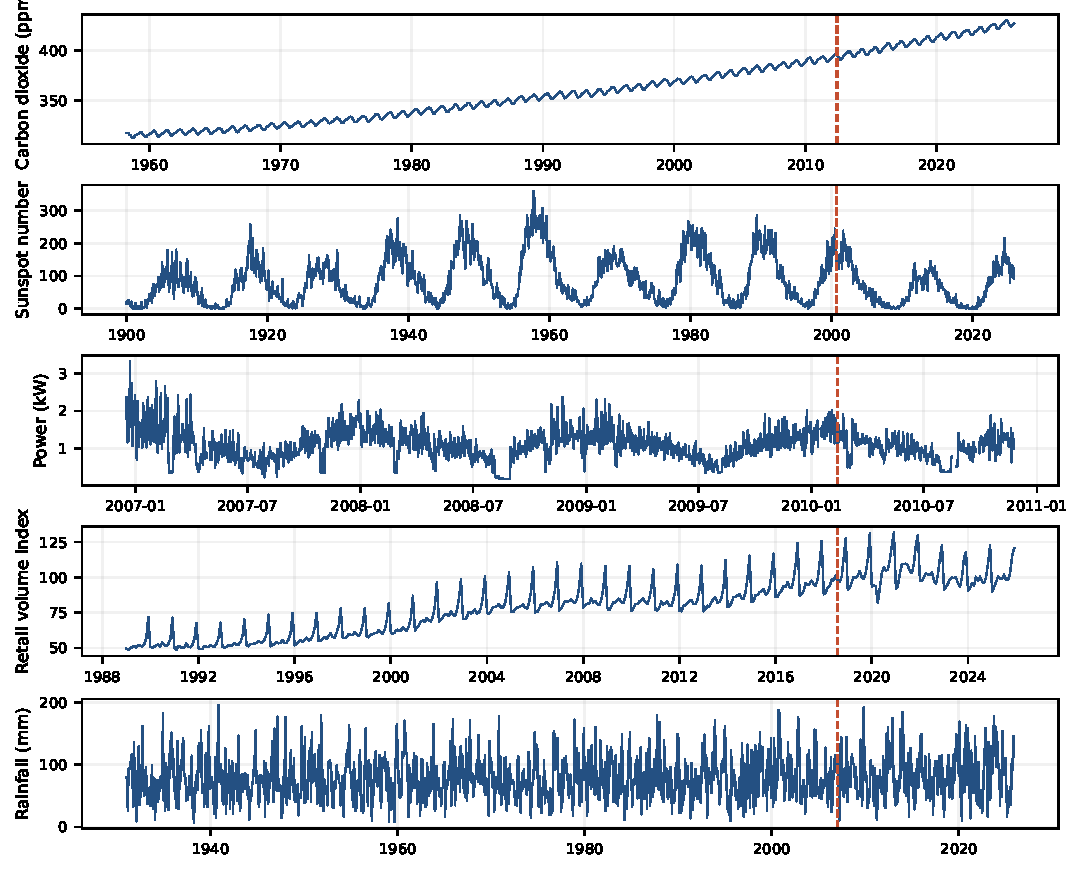
\includegraphics[width=\textwidth]{series.pdf}
\caption{Five observed target levels. The dashed line in each panel marks its final-test boundary. Panels retain their original units and separate vertical scales.}
\label{fig:series}
\end{figure*}

The panels show a rising carbon-dioxide level, changing sunspot-cycle amplitude, variable daily power, changing retail volume, and highly variable rainfall. The figure supports the planned diversity of series. It does not, by itself, establish stationarity or identify the cause of a subsequent forecast error.

Table~\ref{tab:data} reports the modelled lengths and development-only diagnostic results. The ADF and KPSS probabilities were interpreted alongside the observed temporal patterns. The household daily target was the arithmetic mean of valid minute-level active-power measurements, expressed in kilowatts. A day required at least 1,368 valid minutes, or 95\% of the expected 1,440. Incomplete endpoints were excluded. Twenty-three interior days failed the threshold. A missing day was neither fitted nor scored. Model inputs for such days used only the latest \emph{earlier} observed daily value. The rule preserves the daily grid, but it can obscure a change during an outage.

\begin{table*}[t]
\caption{Selected series and development-period level diagnostics}
\label{tab:data}
\centering\small
\begin{tabular}{lrrrlll}
\toprule
Series & Length & Frequency & Missing & Test begins & ADF $p$ & KPSS $p$ \\
\midrule
Carbon dioxide & 813 & month & 0 & 2012-06-01 & $\geq 0.10$ & $\leq 0.01$ \\
Sunspots & 1,512 & month & 0 & 2000-10-01 & $\leq 0.01$ & 0.056 \\
Household power & 1,440 & day & 23 & 2010-02-11 & 0.028 & $\geq 0.10$ \\
Retail volume & 444 & month & 0 & 2018-08-01 & $\geq 0.10$ & $\leq 0.01$ \\
Precipitation & 1,140 & month & 0 & 2007-01-01 & $\leq 0.01$ & $\geq 0.10$ \\
\bottomrule
\end{tabular}
\end{table*}


The carbon-dioxide level rose in the development period. A first difference, $y_t-y_{t-1}$, supplied the network target; the preceding observed level reconstructed the forecast. The source's six post-1974 interpolated months remained in the acquired series and were disclosed rather than silently replaced. The NOAA source also combined early Scripps measurements with later NOAA measurements and substituted a nearby site during the 2022--2023 Mauna Loa interruption. Those source changes limit physical interpretation of forecast errors. The retail level combined long-run rise and annual seasonality. A twelve-month difference, $y_t-y_{t-12}$, removed much of the repeated calendar pattern; the observed level from twelve months earlier reconstructed the forecast. The transformed retail stationarity tests did not agree, so no claim of established stationarity follows. Sunspot, power, and precipitation levels were retained. Source values at zero were valid observations, not missing markers.

For each fold, scaling parameters came only from its fitting prefix. The chronological early-stopping and validation segments used the same fixed scaler. The final refit used a new scaler fitted on the complete development period. Difference lags were fixed before primary fitting. Every reported error was calculated after inverse scaling and, where needed, inverse differencing. No full-series scaler, future-assisted interpolation, or test-fitted decomposition was used.

\section{Implementation}
The implementation account distinguishes the mathematical recurrences from the software used to calculate gradients and manage experiments. Three separate PyTorch modules implement the equations above with explicit linear maps. No built-in recurrent cell supplies the hidden or output feedback. Matrix shapes, parameter counts, initial states, and state updates were checked against hand-computed examples. A single scalar enters each step, and only the final step of a history window contributes a one-step training loss. Observed windows can overlap, but no recurrent state carries between windows.

Training minimised mean squared error on the scaled target with Adam \cite{kingma2015adam}. Gradients were clipped at Euclidean norm one. Hidden weights, output weights, and biases were all trainable; weight decay was fixed at $10^{-4}$. Fixed chronological batches contained at most 256 windows. The three prescribed seeds controlled initial weights and were identical for all architectures. Deterministic central processing unit (CPU) operations were requested, and a repeated pilot run produced identical predictions in the tested environment. Exact software versions, raw hashes, configurations, fold outputs, and seed-level predictions were saved alongside the analysis.

\section{Empirical Process}
The empirical process establishes the chronological boundaries, tuning grid, stopping criterion, and final decision rule. The pilot was a development-only pipeline check and did not contribute to the final comparison. The frozen protocol preceded the primary experiment.

\subsection{Chronological Boundaries}
For a modelled series of length $N$, the development endpoint was $D=\lfloor0.8N\rfloor$. The final test consisted of positions $[D,N)$. A validation block contained $V=\lfloor0.1N\rfloor$ target positions. The three expanding validation intervals were $[D-3V,D-2V)$, $[D-2V,D-V)$, and $[D-V,D)$. The corresponding training intervals began at the first modelled observation and ended before each validation block. The final 10\% of each training interval was reserved as a chronological early-stopping tail. The preceding observations fitted network weights and scaler parameters. Table~\ref{tab:splits} gives the resulting calendar boundaries. Validation target blocks and the final test were disjoint. Their history windows legitimately shared earlier observed inputs.

\begin{table*}[t]
\caption{Start dates of the three validation blocks and final test}
\label{tab:splits}
\centering\small
\begin{tabular}{lllllr}
\toprule
Series & First block & Second block & Third block & Test & Test positions \\
\midrule
Carbon dioxide & 1992-03-01 & 1998-12-01 & 2005-09-01 & 2012-06-01 & 163 \\
Sunspots & 1963-01-01 & 1975-08-01 & 1988-03-01 & 2000-10-01 & 303 \\
Household power & 2008-12-06 & 2009-04-29 & 2009-09-20 & 2010-02-11 & 288 \\
Retail volume & 2007-08-01 & 2011-04-01 & 2014-12-01 & 2018-08-01 & 89 \\
Precipitation & 1978-07-01 & 1988-01-01 & 1997-07-01 & 2007-01-01 & 228 \\
\bottomrule
\end{tabular}
\end{table*}


At each validation or test origin, a model received the latest declared history of observed transformed targets. The history comprised 24 months for carbon dioxide, retail, and precipitation, 60 months for sunspots, and 28 days for power. A target already observed at an earlier origin could enter a later history window. No validation or test target controlled a scaler, preceding forecast, checkpoint, hyperparameter, or final refit epoch before the permitted selection stage. Missing power targets were excluded using one common target mask for all methods.

\subsection{Control Selection and Stopping}
Each architecture searched two approximate capacity budgets and learning rates 0.003 and 0.01. Elman and combined networks used $H\in\{8,18\}$; Jordan used $H\in\{24,96\}$. The parameter budgets were approximately 100 and 400, as calculated from the equations. The same three validation blocks and seeds 11, 23, and 37 were used for every candidate. The search therefore contained four candidate configurations and nine fold-seed evaluations per candidate for each architecture and dataset. The selected configuration had the lowest mean validation MAE. Exact numerical ties favoured fewer trainable parameters and then the lower learning rate. The finite grid supports a best-within-grid conclusion only.

Early stopping selected the checkpoint with the lowest MAE on the chronological tail of the current fold-training interval. Patience was 20 epochs, with a 400-epoch maximum. Training and tail histories were retained to distinguish early stopping from cap-limited training. Once a configuration was selected, its nine best epochs supplied a rounded median fixed epoch count. The model was then refitted on all development observations for each seed. All fifteen architecture-dataset choices were saved before any final-test score was calculated.

\subsection{Evaluation and Evidence Roles}
Primary evaluation compared seed-level MAE on identical final targets. RMSE and MASE assessed large errors and cross-series scaling. Persistence and seasonal-naive forecasts used the same target positions. Fold-level validation records described selection and its sensitivity to origin. Final seed spread described optimisation variation; seed runs did not create independent test periods. A lowest mean test MAE identified the observed winner, while the baseline comparison and paired origin errors bounded practical interpretation. No final-test error changed a configuration.

The pilot verified source loading, split indices, training-only scaling, causal missing inputs, inverse differencing, recurrent-state arithmetic, checkpoint restoration, metrics, saved settings, and a deterministic rerun. Its files were isolated under \texttt{output/pilot}. The primary selection and final evaluation were stored under \texttt{output/primary}; development-only diagnostics were stored under \texttt{output/diagnostics}. Table~\ref{tab:experiments} defines the role and limitation of each experiment before the corresponding results are presented.

\begin{table*}[t]
\caption{Experiment roles fixed before final evaluation}
\label{tab:experiments}
\centering\footnotesize
\begin{tabular}{lllll}
\toprule
Experiment & Partition & Varied factor & Selection role & Main limitation \\
\midrule
Pipeline pilot & CO$_2$ development fold 1 & Network and seed & None & Pipeline check only \\
Control search & Three validation blocks & Capacity and rate & Select settings & Finite grid \\
Final comparison & Final chronological test & Network and seed & Conclusion only & One test period \\
Baseline comparison & Same final targets & Forecast rule & Interpretation only & Reference choice \\
Training curves & Development histories & Epoch & Explanation only & Descriptive only \\
\bottomrule
\end{tabular}
\end{table*}


\section{Results and Discussion}
The results first examine the selected controls, then compare final errors and baselines across the five datasets. The final paragraphs connect observed patterns to data behaviour and identify limits of the comparison.
\subsection{Observed Series and Validation Conditions}
The development-only diagnostics in Table~\ref{tab:data} agree with several visible patterns in Fig.~\ref{fig:series}. For carbon-dioxide levels, the ADF test did not reject a unit root, whereas KPSS rejected level stationarity. A first difference gave ADF $p<0.001$ and KPSS $p\geq0.10$. Retail levels showed the same opposing level-test outcomes. A twelve-month retail difference gave ADF $p=0.158$ and KPSS $p\geq0.10$; this did not establish stationarity. Rainfall gave ADF $p<0.001$ and KPSS $p\geq0.10$, consistent with an approximately stationary level over development. Sunspot levels gave ADF $p<0.001$ but KPSS $p=0.056$, while the plot revealed large amplitude changes between cycles. Power gave ADF $p=0.028$ and KPSS $p\geq0.10$; 23 missing daily targets still required the common causal-input rule. These results justified the declared transformations and cautioned against interpreting a single test as a complete description of a series. The five panels do not, by themselves, identify the mechanism of any later forecast error.

The split dates in Table~\ref{tab:splits} also matter for interpretation. The retail test began in August 2018 and included the sharp 2020--2021 movement visible in Fig.~\ref{fig:series}. The household test occupied only the last part of a roughly four-year record. Accordingly, the retail result tested a marked later disturbance, whereas the power result tested a comparatively short historical interval. Neither interval represents every plausible future operating condition.

\subsection{Selected Controls and Development Variation}
Table~\ref{tab:selection} reports the settings selected without consulting the final periods. The larger capacity budget was chosen in 13 of the 15 architecture-series combinations. The two small-budget choices were Elman for retail and Jordan for rainfall. No selected fold-seed fit had its best checkpoint at the 400-epoch cap.

\begin{table*}[t]
\caption{Selected controls from expanding development validation}
\label{tab:selection}
\centering\small
\begin{tabular}{llrrrrrr}
\toprule
Series & Network & Width & Parameters & Rate & Validation MAE & Refit epochs & Cap fits \\
\midrule
Carbon dioxide & Elman & 18 & 379 & 0.003 & 0.256 & 286 & 0 \\
Carbon dioxide & Jordan & 96 & 385 & 0.010 & 0.575 & 69 & 0 \\
Carbon dioxide & Combined & 18 & 397 & 0.010 & 0.270 & 64 & 0 \\
Sunspots & Elman & 18 & 379 & 0.010 & 18.993 & 14 & 0 \\
Sunspots & Jordan & 96 & 385 & 0.010 & 18.922 & 10 & 0 \\
Sunspots & Combined & 18 & 397 & 0.010 & 18.993 & 11 & 0 \\
Power & Elman & 18 & 379 & 0.010 & 0.212 & 17 & 0 \\
Power & Jordan & 96 & 385 & 0.010 & 0.219 & 28 & 0 \\
Power & Combined & 18 & 397 & 0.010 & 0.212 & 15 & 0 \\
Retail & Elman & 8 & 89 & 0.010 & 1.395 & 19 & 0 \\
Retail & Jordan & 96 & 385 & 0.010 & 1.383 & 12 & 0 \\
Retail & Combined & 18 & 397 & 0.003 & 1.427 & 14 & 0 \\
Rainfall & Elman & 18 & 379 & 0.010 & 29.427 & 12 & 0 \\
Rainfall & Jordan & 24 & 97 & 0.003 & 29.695 & 8 & 0 \\
Rainfall & Combined & 18 & 397 & 0.003 & 29.790 & 17 & 0 \\
\bottomrule
\end{tabular}
\end{table*}


The selected carbon-dioxide Elman network used 379 parameters, rate 0.003, and 286 refit epochs. Jordan used 385 parameters, rate 0.01, and 69 epochs; the combined network used 397 parameters, rate 0.01, and 64 epochs. Similar parameter counts did not produce similar validation MAE: Elman and combined feedback obtained 0.256 and 0.270 ppm, respectively, compared with Jordan's 0.575 ppm. The difference is consistent with a useful hidden-state feedback path for this transformed seasonal series, although capacity matching does not isolate feedback as a causal mechanism. Jordan's 96 hidden units also yielded a different optimisation geometry from Elman's 18.

Validation origins exposed temporal variation that a single aggregate would hide. Sunspot Elman mean MAE rose from 14.857 in the first block to 21.108 and 21.013 in the next two. Power Elman moved from 0.261 to 0.160 and 0.214 kW. Retail Elman moved from 1.515 to 1.278 and 1.392 index points. The three retail network means differed by only 0.044 index points at selection. These changes indicate that performance depended on the calendar interval, so a small overall selection advantage should not be read as a stable ordering across origins. The fixed three-block design measures that sensitivity only at the chosen boundaries.

The final retail MAEs were much larger than the development validation means in Table~\ref{tab:selection}. Jordan's 1.383 validation MAE preceded a 3.416 test MAE. The test period included the large retail movements visible in Fig.~\ref{fig:series}; this association supports a distribution-shift explanation but does not quantify a causal contribution of any specific event. Sunspot Elman moved in the other direction, from 18.993 development validation MAE to 13.413 test MAE. Thus validation selected controls, but it was not an unbiased prediction of error in every later period.

The saved development curves supplied a supplementary check on early stopping, as declared in Table~\ref{tab:experiments}. Among 135 selected-configuration fold-seed fits, 131 had lower scaled training loss at the final trained epoch than at the checkpoint selected by chronological-tail MAE. The final tail MAE was no lower than the selected minimum by construction. Continuing reduction in training loss alongside the lack of tail improvement supports the use of early stopping in this protocol. It does not isolate overfitting: the two measures use different metrics, and the tail is a later calendar interval. This diagnostic did not alter any selected configuration.

\subsection{Primary Architecture Comparison}
Table~\ref{tab:performance} gives original-unit final errors for all three required architectures. MAE is the prespecified ranking measure. RMSE and MASE provide supporting views of large errors and cross-series scale. The displayed standard deviation concerns the three initialisation seeds, not independent test periods.

\begin{table*}[t]
\caption{Final-period network errors averaged across three initialisation seeds}
\label{tab:performance}
\centering\small
\begin{tabular}{llrrr}
\toprule
Series & Network & MAE $\pm$ seed SD & RMSE & MASE \\
\midrule
Carbon dioxide & Elman & $0.328\pm0.003$ & 0.414 & 0.305 \\
Carbon dioxide & Jordan & $0.658\pm0.013$ & 0.850 & 0.612 \\
Carbon dioxide & Combined & $0.324\pm0.006$ & 0.399 & 0.302 \\
Sunspots & Elman & $13.413\pm0.100$ & 18.743 & 0.667 \\
Sunspots & Jordan & $14.366\pm0.465$ & 19.603 & 0.715 \\
Sunspots & Combined & $13.512\pm0.132$ & 18.959 & 0.672 \\
Power & Elman & $0.169\pm0.002$ & 0.236 & 0.586 \\
Power & Jordan & $0.196\pm0.027$ & 0.254 & 0.681 \\
Power & Combined & $0.173\pm0.003$ & 0.240 & 0.598 \\
Retail & Elman & $3.457\pm0.030$ & 5.138 & 0.662 \\
Retail & Jordan & $3.416\pm0.120$ & 5.121 & 0.654 \\
Retail & Combined & $3.495\pm0.040$ & 5.237 & 0.670 \\
Rainfall & Elman & $30.009\pm0.527$ & 37.227 & 0.801 \\
Rainfall & Jordan & $31.454\pm0.180$ & 38.724 & 0.840 \\
Rainfall & Combined & $30.885\pm0.469$ & 38.088 & 0.825 \\
\bottomrule
\end{tabular}
\end{table*}


For carbon dioxide, combined feedback had the lowest MAE, 0.324 ppm, and RMSE, 0.399 ppm. Elman followed at 0.328 and 0.414 ppm; Jordan reached 0.658 and 0.850 ppm. The combined MAE advantage over Elman was 0.00354 ppm, or 1.08\% of Elman's MAE, smaller than the seed standard deviations of 0.006 and 0.003 ppm. Both hidden-feedback networks may exploit short-run information in the first-differenced input that output feedback alone represented less effectively in this implementation. This interpretation is conditional on the chosen widths and optimisation procedure; the test does not prove that one feedback path is inherently superior.

For sunspots, Elman gave the lowest MAE, 13.413 sunspots, followed by combined feedback at 13.512 and Jordan at 14.366. The Elman--combined difference was 0.099, close to their seed standard deviations of 0.100 and 0.132. The varying cycle amplitude and occasional abrupt monthly changes in Fig.~\ref{fig:series} limit what a fixed 60-month observed history can explain. The measured ordering therefore supports a modest Elman lead on this period, not a reliable hierarchy across solar cycles.

For power, Elman obtained 0.169 kW MAE and 0.236 kW RMSE. Combined feedback obtained 0.173 and 0.240 kW; Jordan obtained 0.196 and 0.254 kW. Jordan's MAE seed standard deviation, 0.027 kW, was much larger than Elman's 0.002 and combined feedback's 0.003 kW. The result suggests greater sensitivity of the selected Jordan fit to initialisation on this series. Missing days and the short test interval restrict extrapolation to other households and seasons.

Retail reversed the broad pattern: Jordan had the lowest observed MAE, 3.416 index points, and RMSE, 5.121. Elman followed at 3.457 and 5.138, with combined feedback at 3.495 and 5.237. Jordan's advantage over Elman was 0.0416 index points, or 1.20\% of Elman's MAE, while Jordan's seed standard deviation was 0.120. The twelve-month difference represented the established annual pattern, and the later sharp movement made level reconstruction demanding. The narrow gap and larger Jordan seed spread prevent a strong claim of Jordan superiority on retail beyond this test interval.

For precipitation, Elman gave the lowest MAE and RMSE, 30.009 and 37.227 mm. Combined feedback gave 30.885 and 38.088 mm; Jordan gave 31.454 and 38.724 mm. Large month-to-month variation remained in the level series even though the development stationarity diagnostics were compatible with a stable mean. Such variability plausibly limits the benefit of learned recurrent memory. The data cover one regional rainfall aggregate, and the comparison cannot establish that the same ordering holds for other locations or accumulation periods.

\subsection{Practical Skill Against Diagnostic Forecasts}
Table~\ref{tab:baselines} reports baseline errors on exactly the target positions used in Table~\ref{tab:performance}. Figure~\ref{fig:skill} shows each network MAE divided by the corresponding persistence MAE. A ratio below one means a lower error than persistence. The figure supports comparisons across units while retaining all three architectures.

\begin{table}[t]
\caption{Final-period diagnostic MAE in original units}
\label{tab:baselines}
\centering\footnotesize
\begin{tabular}{lrrr}
\toprule
Series & Targets & Persistence & Seasonal \\
\midrule
Carbon dioxide & 163 & 1.211 & 2.546 \\
Sunspots & 303 & 14.219 & -- \\
Power & 276 & 0.199 & 0.245 \\
Retail & 89 & 7.069 & 3.978 \\
Rainfall & 228 & 39.574 & 42.041 \\
\bottomrule
\end{tabular}
\end{table}


\begin{figure*}[t]
\centering
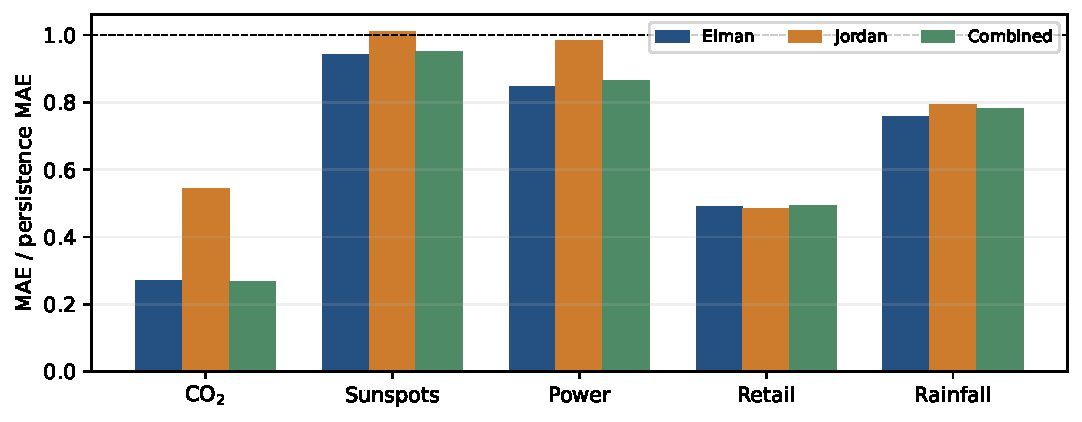
\includegraphics[width=0.82\textwidth]{skill.pdf}
\caption{Final-test network MAE relative to persistence MAE. The horizontal line denotes equal error. Lower ratios are better.}
\label{fig:skill}
\end{figure*}

The best neural forecast improved on persistence by 73.21\% for carbon dioxide, 5.67\% for sunspots, 15.26\% for power, 51.67\% for retail, and 24.17\% for rainfall. Retail's applicable seasonal-naive method was stronger than persistence, at 3.978 rather than 7.069 index points MAE. Against that stronger baseline, Jordan's retail improvement was 14.12\%. Seasonal-naive was weaker than persistence for carbon dioxide, power, and rainfall. Jordan sunspots had 14.366 MAE, which exceeded persistence's 14.219; the required architecture did not always add practical skill. The absence of a fixed seasonal-naive solar benchmark follows from its variable cycle rather than from a zero baseline error. These ratios depend on the chosen diagnostic rules and do not measure economic or operational value.

MASE supplies a second scale-independent check. The best network's final MASE was 0.302 for carbon dioxide, 0.667 for sunspots, 0.586 for power, 0.654 for retail, and 0.801 for rainfall. Each value was below one relative to the training-period first-difference scale. A MASE below one here means that the model's test MAE was below that fixed training reference; it does not mean that it beat every test-period naive method. In particular, retail's seasonal baseline and sunspots' persistence should be read directly from Table~\ref{tab:baselines}. The five denominators were estimated from different histories and are not interchangeable measures of task difficulty.

\subsection{Representative Forecast Behaviour and Limits}
Figure~\ref{fig:examples} shows the final 70 scored target positions for carbon dioxide and retail using the lowest-mean-MAE architecture in each case. Each blue line averages the three seed forecasts for display only; Tables~\ref{tab:performance} and \ref{tab:baselines} use the saved seed-level forecasts. This post-hoc display illustrates where a small average error may coexist with larger individual misses and did not affect selection.

\begin{figure*}[t]
\centering
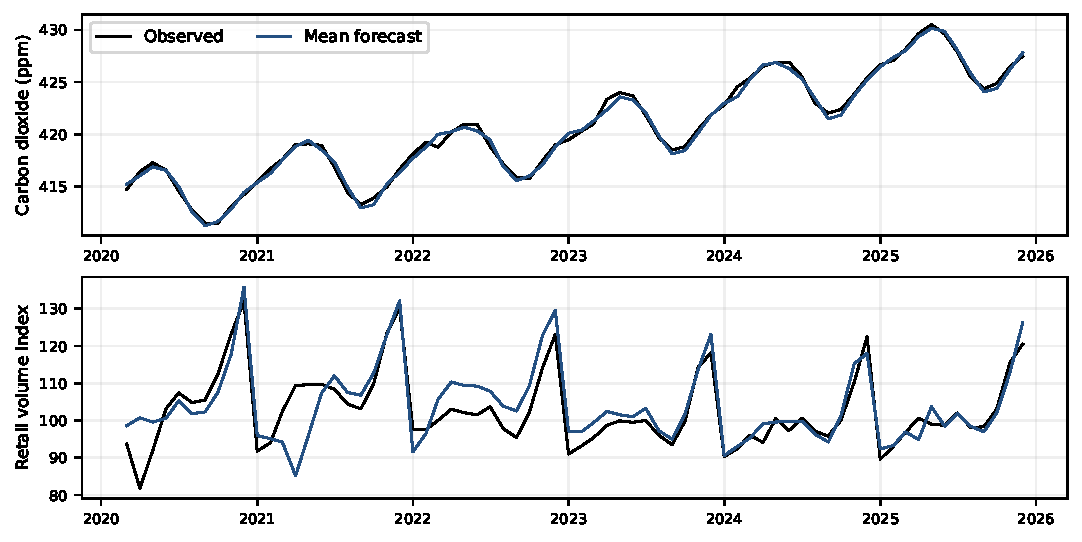
\includegraphics[width=0.86\textwidth]{examples.pdf}
\caption{Observed levels and mean forecasts for the final 70 scored carbon-dioxide and retail targets. The selected combined network is shown for carbon dioxide and Jordan for retail.}
\label{fig:examples}
\end{figure*}

The carbon-dioxide panel tracks the rising observed level while retaining some monthly error. The retail panel shows larger misses around sharp changes, consistent with its RMSE of 5.121 exceeding its MAE of 3.416. The largest retail absolute error in one displayed seed was 24.28 index points in April 2021. This outlier illustrates how a changing level can dominate squared-error measures, but a single miss does not establish the general cause of error. The panels omit earlier test origins and show a seed-mean trajectory; they should not be treated as independent or additional evaluations.

The cross-series evidence supports a narrower conclusion than a universal winning architecture. Elman had the lowest observed MAE on three series, combined feedback on one, and Jordan on one. The combined path never produced a large final advantage over Elman under the frozen grid, even though it added trainable weights. Conversely, the larger Elman--Jordan differences on carbon dioxide and power showed that nominally similar parameter counts did not guarantee similar predictions. The finite architecture-specific search, three seeds, fixed input histories, and one final period per series limit the generality of both statements. Repeated origins within a series were temporally dependent, so the study did not treat their errors as independent samples for a significance test.


\clearpage

\section{Conclusions}
The study compared Elman hidden feedback, Jordan predicted-output feedback, and combined feedback for one-step forecasts of five series. Under the frozen chronological protocol, combined feedback had the lowest carbon-dioxide mean absolute error (MAE), 0.324 ppm; Elman had the lowest MAE for sunspots (13.413), household power (0.169 kW), and rainfall (30.009 mm); Jordan had the lowest retail MAE (3.416 index points). The carbon-dioxide and retail leads over Elman were about 1\%, so those observed winners were qualified by seed variability. The best network on each series improved on its strongest applicable naive forecast by 5.7\%--73.2\%. No feedback architecture dominated all datasets. These findings were limited to the declared histories, two capacity budgets, two learning rates, three seeds, and one historical test period per series. A future study could repeat the frozen comparison across additional later periods and regions, with search budgets expanded equally and all new selections confined to their earlier development periods.


\appendices
\section{Acronyms}
\begin{tabular}{ll}
ADF & augmented Dickey--Fuller\\
KPSS & Kwiatkowski--Phillips--Schmidt--Shin\\
MAE & mean absolute error\\
MASE & mean absolute scaled error\\
RMSE & root mean squared error\\
SRNN & simple recurrent neural network
\end{tabular}

\section{Mathematical Symbols}
\begin{tabular}{ll}
$D$ & development endpoint\\
$e_i$ & level-unit forecast error\\
$H$ & hidden-layer width\\
$m$ & number of scored origins\\
$N$ & modelled series length\\
$t$ & time index\\
$V$ & validation-block length\\
$y_t$ & observed target\\
$z_t$ & transformed, scaled observation\\
$\mathbf h_t$ & hidden state\\
$\mathbf W_x,\mathbf W_h,\mathbf W_o,\mathbf W_y$ & trainable weight matrices\\
$\mathbf b_h,b_y$ & trainable biases
\end{tabular}

\bibliographystyle{IEEEtranS}
\bibliography{../citations/references}
\end{document}
